\chapter{Conclusion}
\label{chap:conclusion}

\minitoc

\graphicspath{{.}{chapitres/conclusion/}}

\section{Contributions Summary}
\label{sec:conclusion:contributions-summary}

\subsection{\dspot}
\label{subsec:conclusion:contributions-summary:dspot}

The major technical contribution of this thesis is \dspot, a unit test methods amplification tool.
\dspot aims at improving existing test method with respect to an given test-criterion such as branch coverage.
It does this in 3 main steps.

1) It amplifies the input of the original test method by applying specific code transformation on the input part of the test method;

2) It removes existing assertions and generates new ones, based on observations done during execution on the state of the programs.
It uses commons getters in Java to do so, \eg non-void methods with no parameter that starts with ``get'';

3) It uses a test-criterion to select amplified test methods to keep.
For instance, one want to improve the branch coverage of the test suite.
\dspot will keep only amplified test methods that cover branches that were not cover before.

\dspot has been developed in Java, for Java programs.
However, the whole technique remains applicable for all programming languages.

All the code of \dspot is available on \gh: \url{https://github.com/STAMP-project/dspot.git}.
I personally enliven its community by answering questions on the bug tracker, guiding new contributors and setting up developing methodologies , such as pull-request based developers or integration continue, to keep \dspot as clean as possible.


Following this technical contribution, this thesis presented two large-scale evaluations of \dspot's effectiveness.

\subsection{Automatic Test Amplification For Mutation Score}
\label{subsec:conclusion:contributions-summary:test-ampl-ms}

For a first evaluation, I used \ms as test-criterion.
\dspot has automatically amplified test suites from open-source projects from \gh and improve the \ms.
\ms has been used as a proxy of test suites' ability to detect faults.

The outputted amplified test methods of \dspot have been proposed to external developers of the projects from \gh through pull-requests.
This has been done in order to have the developers assessing the result of \dspot.
Over 19 opened pull-requests, 14 of them have been permanently added to the test suites of these projects.
It means that \dspot generated amplified test methods that are valuables for external developers.
Everyday, amplified test methods are increasing the developers' confidence in the correctness of their software.

Also, I evaluated \dspot in a more ``off-line'' way by amplifying 40 test classes of heavily tested projects from \gh, using also the \ms as test-criterion.
This evaluation that \dspot is able to generate amplified test methods that increase \ms.

\subsection{Automatic Test Amplification For Behavioral Changes Detection}
\label{subsec:conclusion:contributions-summary:behavioral-change-detection}

In a second evaluation, I used \dspot in the context of continuous integration.
The goal is to generate amplified test methods that detect behavioral changes.

I took open-source projects from \gh and a commits selection.
This evaluation showed that \dspot is able to generate amplified test methods that detect 25 behavioral change over 40.
It also highlights the fact that \dspot can be easily implemented in the life cyle of software, like continuous integration.

This evaluation brings evidence that \dspot has to potential to be a concrete part of continuous integration by improving the process of program evolution with amplified test methods that are able to distinguish between versions of the same program.

\subsection{Transversal Contributions}
\label{subsec:conclusion:contributions-summary:transversal-contributions}

During this thesis, I developed a wide range of knowledge and skills that allowed me to participated to diversified and transversal contributions.

\subsubsection{Study of Program Correctness}
\label{subsubsec:conclusion:contributions-summary:transversal-contributions:correctness-attraction}

I devised a protocol, named \perturb, to study the programs' correctness under runtime perturbation.
10 subjects have been studied using the PONE perturbations model, \ie adds 1 to integer expression at runtime.
It results in 2509012 perturbed executions, which makes it one of the largest perturbation experiments ever made.
From this experimentation, the presence of ``correctness attraction'' has been observed. 
Over all perturbed execution, 66\% of them do not break the correctness of the output. 

\subsubsection{Study of Pseudo-tested Methods}
\label{subsubsec:conclusion:contributions-summary:transversal-contributions:pseudo-tested}

We replicated the study of \theoriginalauthors and confirmed that all Java projects contain \pseudotested{} methods, even the very well tested ones, ranging from 1\% to 46\% in our dataset.
From 3 projects, developers consider that 30\% methods were worthy of additional testing actions.

\subsubsection{Study of Test Generation for Repair}
\label{subsubsec:conclusion:contributions-summary:transversal-contributions:test-for-repair}

To sum up, UnsatGuided can effectively alleviate the overfitting issue of regression introduction (16/19 cases), but has minimal positive impact on reducing the overfitting issue of incomplete fixing.

In this study, we used Evosuite, a state-of-the-art test generation tool.
An alternative would be to use a test amplification tool, such as \dspot in order to overcome the overfitting problems.

\section{Short-term perspectives}
\label{sec:conclusion:short-prespectives}

In this section, I introduce short-perspectives for \dspot.

1) Even if amplified test methods are based on existing ones, they are still automatically produced resulting that they might be difficult to read and understand.
A first key-feature is to make them ``prettier'', and \autoref{subsec:conclusion:short-prespectives:prettifier} introduces a way to do it.

2) and a web interface, introduced in \autoref{subsec:conclusion:short-prespectives:web-interface} that allows developers to execute \dspot, inspired by guru.io.

\subsection{DSpot-prettifier}
\label{subsec:conclusion:short-prespectives:prettifier}

\dspotprettifier is a maven plugin for DSpot that aims at prettifying the amplified test methods.
\dspotprettifier takes as input a set of ``ugly'' amplified test methods and a test-criterion to output a set of ``prettier'' amplified test methods.
It ensures that the outputted amplified test methods have the same quality than the input amplified test methods, with respect to the given test-criterion, \eg \ms.

It works in 3 main steps:

1) it minimizes the number of statement(\autoref{subsubsec:conclusion:short-prespectives:prettifier:miminize});

2) it renames all the local variables with a name according to the context(\autoref{subsubsec:conclusion:short-prespectives:prettifier:rename-local});

3) it renames the amplified test methods according to its body(\autoref{subsubsec:conclusion:short-prespectives:prettifier:rename-method}).

This workflow is summarize in \autoref{fig:dspot-prettifier-overview}.

\begin{figure}
	\label{fig:dspot-prettifier-overview}
	\caption{Overview of DSpot-prettifier's approach}
	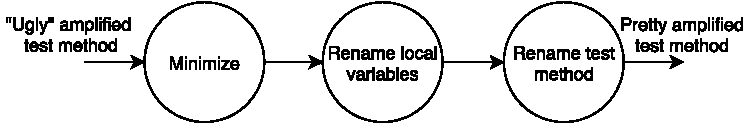
\includegraphics[width=.9\linewidth]{approach.pdf}
\end{figure}

\subsubsection{Minimization}
\label{subsubsec:conclusion:short-prespectives:prettifier:miminize}
The minimization step aims at reducing the size of the statement and the number statement to the minimal.
This is done in 2 majors steps:

1) modifying the code using static analysis to avoid redundancy or useless local variable declaration;
\dspotprettifier replaces multiple method calls, \eg to getters, that are the same by a local variable.
In the other way, it replaces local variables that are used only one time.

2) applying a search-based algorithm to remove the maximum number of statements, \emph{w.r.t.} to the specified test-criterion.
The intuition is as follow:
\dspotprettifier removes one statement;
it tries to compile the new test method;
if it fails, it means that this statement is needed to compile the test method and it must keep it;
otherwise, it measure the quality of the new test method according to the test criterion;
if it remains the same, \dspotprettifier can remove the statement definitively, otherwise it cannot be removed;
It repeats this process for all the statement inside the test method, starting by the end of the body.

A proof-of-concept implementation for \ms has been done.

\subsubsection{Rename local variables}
\label{subsubsec:conclusion:short-prespectives:prettifier:rename-local}

The second step of the prettifying algorithm is to rename the local variables.
To do this, \dspotprettifier could use Context2Name\footnote{\url{https://github.com/rbavishi/Context2Name}}\cite{DBLP:journals/corr/abs-1809-05193} which is a deep learning-based approach to infer natural variable names from usage contexts.

\subsubsection{Rename amplified test method}
\label{subsubsec:conclusion:short-prespectives:prettifier:rename-method}

The second step of the prettifying algorithm is to rename the local variables.
To do this, \dspotprettifier could use Code2Vec\footnote{\url{https://github.com/tech-srl/code2vec}}\cite{DBLP:journals/corr/abs-1803-09473} which is a neural network for learning distributed representations of code.

A first proof-concept implementation is avalaible on \url{https://github.com/STAMP-project/dspot/tree/master/dspot-prettifier}.

\subsection{DSpot web interface}
\label{subsec:conclusion:short-prespectives:web-interface}
The idea is to provide to users a web interface, on which the user would have simply to put the URL of its \gh repository.
Then, we retrieve the project and run \dspot on it.
This idea is largely inspired by CommitGuru\footnote{\url{http://commit.guru/}}\cite{Rosen:2015:FSE}.

There is already a first proof-of-concept avalaible: \url{http://dspot.kth-assert.net/}.

For now, the user cannot configure \dspot as he desired.
\dspot is executed on the project with the default configuration.
A challenge is to detect automatically how the project is organized: modules, source folders, etc.
However, the goal of this web interface is to allow new users discover \dspot and its capability.
For now, users receive the result of the amplification through email notification, but we could imagine a complete dashboard that report \dspot executions.

A screenshot of the web interface is shown in \autoref{fig:dspot-web} and an example of the report provided by the web interface after a successful amplification \autoref{verbatim-example-report-dspot-web}.

\section{Long-term perspectives}
\label{sec:conclusion:long-prespectives}

In my vision, there are 2 long-term perspectives for \dspot:

1) sometimes, test-improvement resulting from a given test class should not be in the same class. \eg \autoref{subsubsec:test-improvement:experiment-results:rq1:mustache}.
This might be a limitation on the adoption of \dspot by industrials since they might be confused by the fact that the component tested is not any more related to the original test class.

2) Inspired from Repairnator~\cite{urli:hal-01691496}, we could imagine a bot that uses \dspot in a similar way than Repairnator uses automatic repair tool.
That is to say, the bot would launch \dspot on passing build, a contrario than Repairnator is executed on failing build, to amplify the test suite with to goal to generate amplified test methods that either improve the test suite regarding a changes, or detect a regression introduces by changes.

\section{Conclusion}
\label{sec:conclusion:conclusion}


